\documentclass{beamer}
\usepackage[titlepage=images/titlepage.jpg]{uibkstyle}
\usepackage[utf8]{inputenc}
\usepackage[german]{babel}
\usepackage{graphicx}
\usepackage{subfigure}

\usepackage{tikz}
\usetikzlibrary{decorations.pathmorphing}

\graphicspath{{images/}}

\tikzset{
    onslide/.code args={<#1>#2}{%
        \only<#1>{\pgfkeysalso{#2}}
    },
    month/.style={%
        text depth=.25ex,
        text centered,
    }
}
\tikzset{
    other/.style={circle, onslide=<3-7>{white}}
}

\usetikzlibrary{positioning, arrows, decorations.markings}
\tikzset{%label colors for port states
    port/.style={draw, circle},
    dedicated/.style={port, fill=blue!50},
    root/.style={port, fill=green!50},
    blocking/.style={port, fill=red!50}
}

\tikzset{%used for "invisible" stuff
    invisible/.style={draw=white}
    visible/.style={draw=black}
}

\newcommand{\switch}[2]{
    \scalebox{#1}{
        \begin{tikzpicture}
            \node at (0,0) {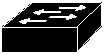
\includegraphics{switch.pdf}};
            \node at (0,-0.6) {#2};
        \end{tikzpicture}
    }
}


\title{STPViz}
\subtitle{Visualizing network topologies with the help of the Spanning Tree Protocol}
\author{Alexander Schlögl}

\begin{document}
\begin{frame}[plain]
    \maketitle
\end{frame}

\begin{frame}{Überblick}
    \begin{itemize}
        \item \textbf{Einleitung \& Motivation}
        \item \textbf{Spanning Tree Protocol (STP)}
        \item \textbf{STPViz}
        \item \textbf{Software-Switch}
        \item \textbf{Tests}
        \item \textbf{Zusammenfassung \& Ausblick}
    \end{itemize}
\end{frame}

\begin{frame}{Überblick}
    \begin{itemize}
        \item \alert{\textbf{Einleitung \& Motivation}}
        \item \textbf{Spanning Tree Protocol (STP)}
        \item \textbf{STPViz}
        \item \textbf{Software-Switch}
        \item \textbf{Tests}
        \item \textbf{Zusammenfassung \& Ausblick}
    \end{itemize}
\end{frame}

\begin{frame}{Warum STP?}
    \begin{itemize}[<+->]
        \item Redundanz in großen Netzwerken erwünscht
        \item Schleifen im Netzwerk entstehen
        \item Das führt zu Broadcast Storms
    \end{itemize}
\end{frame}

\begin{frame}{Broadcast Storms}
    \centering
    \begin{figure}
        \begin{tikzpicture}
            \node (root) at (4,8) {\switch{0.8}{A}};
            \node (B) at (2,6) {\switch{0.8}{B}};
            \node (C) at (6,6) {\switch{0.8}{C}};
            \node (D) at (4,4) {\switch{0.8}{D}};

            \draw
            [onslide=<2>{green, thick, ->},
            onslide=<4>{green,thick, <-},
            onslide=<5>{red,thick,<->}]
            (root) edge (B);

            \draw
            [onslide=<2>{green, thick, ->},
            onslide=<4>{green,thick, <-},
            onslide=<5>{red,thick,<->}]
            (root) edge (C);

            \draw
            [onslide=<3>{red, thick, <->},
            onslide=<5>{red, thick, <->}]
            (B) edge (C);

            \draw
            [onslide=<3>{green, thick, ->},
            onslide=<4-5>{red,thick,<->}]
            (B) edge (D);

            \draw
            [onslide=<3>{green, thick, ->},
            onslide=<4-5>{red,thick,<->}]
            (C) edge (D);
        \end{tikzpicture}
    \end{figure}
\end{frame}

\begin{frame}{Broadcasts mit STP}
    STP deaktiviert doppelte Verbindungen.\\
    Baum Topologie entsteht.
    \pause
    \begin{figure}
        \begin{tikzpicture}
            \node (root) at (4,8) {\switch{0.8}{A}};
            \node (B) at (2,6) {\switch{0.8}{B}};
            \node (C) at (6,6) {\switch{0.8}{C}};
            \node (D) at (4,4) {\switch{0.8}{D}};

            \draw
            [onslide=<+(1)>{green,thick,->}]
            (root) edge (B);

            \draw
            [onslide=<.(1)>{green,thick,->}]
            (root) edge (C);

            \draw
            [onslide=<+(1)>{green,thick,->}]
            (B) edge (D);
        \end{tikzpicture}
    \end{figure}
\end{frame}

\begin{frame}{Grundidee}
    \begin{itemize}[<+->]
        \item Große Netzwerke sind schwer zu administrieren
        \item STP verbirgt Fehler und Änderungen zusätzlich
        \item STP Konfiguration ist komplex
    \end{itemize}
    \pause
    Kommerzielle Tools existieren.\\
    \alert{Aber: Diese nutzen SNMP}
\end{frame}


\begin{frame}{Was waren unsere Ziele?}
    \begin{itemize}[<+->]
        \item Nur STP
        \item Geringe verursachte Netzwerkauslastung
        \item Passiv
        \item Verteilt
        \item Geringe Hardwareauslastung
        \item Keine Instandhaltung notwendig
        \item Mehrere Bäume möglich
    \end{itemize}
\end{frame}

\begin{frame}{Zeitplanung}
    \centering
    \begin{figure}
        \begin{tikzpicture}[month]
            \draw (0,0) -- (0.4,0);
            \draw[->] (0.6,0) -- (10,0);
            %cut marker
            \draw[decorate, decoration={snake,amplitude=1pt,segment length=5pt}] (0.41, 0.3) -- (0.41, -0.3);
            \draw[decorate, decoration={snake,amplitude=1pt,segment length=5pt}] (0.62, 0.3) -- (0.62, -0.3);
            \foreach \x in {0,...,9}
                \draw (\x,0.1) -- (\x,-0.1);

            \node at (0,-0.5) {\tiny Oktober};
            \node at (1,-0.5) {\tiny Februar};
            \node at (2,-0.5) {\tiny März};
            \node at (3,-0.5) {\tiny April};
            \node at (4,-0.5) {\tiny Mai};
            \node at (5,-0.5) {\tiny Juni};
            \node at (6,-0.5) {\tiny Juli};
            \node at (7,-0.5) {\tiny August};
            \node at (8,-0.5) {\tiny September};
            \node at (9,-0.5) {\tiny Oktober};

            \draw (0,0.7) rectangle (1,0.5);\node () at (0.5,1) {\tiny Vorarbeit}; 
            \draw (1,0.7) rectangle (3,0.5);\node () at (2,1) {\tiny Implementation}; 
            \draw (3,0.7) rectangle (3.5,0.5);\node () at (3.25,1) {\tiny Tests};
            \draw (3.5,0.7) rectangle (4.5,0.5);\node () at (4,1) {\tiny Zus. Feat.}; 
            \draw (4.5,0.7) rectangle (5,0.5);\node () at (4.75,1) {\tiny Tests};
            \draw (5,0.7) rectangle (6,0.5);\node () at (5.5,1) {\tiny Arbeit}; 
            \draw[->] (6,1.5) -- (6,0);\node () at (6,1.7) {\tiny Präsentation};
        \end{tikzpicture}
    \end{figure}
\end{frame}

\begin{frame}{Überblick}
    \begin{itemize}
        \item \textbf{Einleitung \& Motivation}
        \item \alert{\textbf{Spanning Tree Protocol (STP)}}
        \item \textbf{STPViz}
        \item \textbf{Software-Switch}
        \item \textbf{Tests}
        \item \textbf{Zusammenfassung \& Ausblick}
    \end{itemize}
\end{frame}

\begin{frame}{STP Funktionsweise}
    Globale Root wird durch Prioritäten bestimmt.\\
    Nur kürzester Pfad zur Root bleibt erhalten.
    \pause
    \begin{figure}
        \begin{tikzpicture}
            \node (root) at (2,2) {\switch{0.8}{Root}};
            \node (a) at (0,0) {\switch{0.8}{A}};
            \node (b) at (4,0) {\switch{0.8}{B}};

            \draw
            (root) -- node[dedicated, at start]{} node[root, at end]{} (a)
            (root) -- node[dedicated, at start]{} node[root, at end]{} (b)
            (a) -- node[dedicated, at start]{} node[blocking, at end]{} (b);

            \begin{customlegend}[legend cell align=left, legend entries={Root Port,Dedicated Port,Blocking Port},
                legend image post style={scale=2.3},
                legend style={at={(8,2)},font=\footnotesize}]
                \addlegendimage{white,mark=*,fill=green}
                \addlegendimage{white,mark=*,fill=blue!80}
                \addlegendimage{white,mark=*,fill=red}
            \end{customlegend}
        \end{tikzpicture}
    \end{figure}
    \pause
    \footnotesize Bemerkung: Wir werden Switches Bridges nennen
\end{frame}

\begin{frame}{STP Pakete}
    \centering
    \begin{figure}
        \begin{tikzpicture}[scale=0.35]
            \foreach \x in {0,...,31}
            \node at (\x+0.5,20.5) {\scriptsize \x};
            \draw (0,20) rectangle (16,18.5); \node (mode) at (8, 19.25) {Protocol Identifier};
            \draw (16,20) rectangle (24,18.5); \node (mode) at (20, 19.25) {Version Id};
            \draw (24,20) rectangle (32,18.5); \node (mode) at (28, 19.25) {BPDU Type};
            \draw[onslide=<+(1)>{red,line width=3pt}] (0,18.5) rectangle (8,17); \node (mode) at (4, 17.75) {Flags};
            \draw[onslide=<+(1)>{red,line width=3pt}] (8,18.5) rectangle (32,17); \node (mode) at (20, 17.75) {Root Identifier};
            \draw[onslide=<.(1)>{red,line width=3pt}] (0,17) rectangle (32,15.5); \node (mode) at (16, 16.25) {Root Identifier};
            \draw[onslide=<.(1)>{red,line width=3pt}] (0,15.5) rectangle (8,14); \node (mode) at (4, 14.75) {Root Identifier};
            \draw (8,15.5) rectangle (32,14); \node (mode) at (20, 14.75) {Root Path Cost};
            \draw (0,14) rectangle (8,12.5); \node (mode) at (4, 13.25) {Root Path Cost};
            \draw[onslide=<+(1)>{red,line width=3pt}] (8,14) rectangle (32,12.5); \node (mode) at (20, 13.25) {Bridge Identifier};
            \draw[onslide=<.(1)>{red,line width=3pt}] (0,12.5) rectangle (32,11); \node (mode) at (16, 11.75) {Bridge Identifier};
            \draw[onslide=<.(1)>{red,line width=3pt}] (0,11) rectangle (8,9.5); \node (mode) at (4, 10.25) {Bridge Identifier};
            \draw (8,11) rectangle (24,9.5); \node (mode) at (16, 10.25) {Port Identifier};
            \draw[onslide=<+(1)>{red,line width=3pt}] (24,11) rectangle (32,9.5); \node (mode) at (28, 10.25) {Message Age};
            \draw[onslide=<.(1)>{red,line width=3pt}] (0,9.5) rectangle (8,8); \node (mode) at (4, 8.75) {Message Age};
            \draw (8,9.5) rectangle (24,8); \node (mode) at (16, 8.75) {Max Age};
            \draw (24,11) rectangle (32,8); \node (mode) at (28, 8.75) {Hello Time};
            \draw (0,8) rectangle (8,6.5); \node (mode) at (4, 7.25) {Hello Time};
            \draw (8,8) rectangle (24,6.5); \node (mode) at (16, 7.25) {Forward Delay};
        \end{tikzpicture}
    \end{figure}
\end{frame}

\begin{frame}{Überblick}
    \begin{itemize}
        \item \textbf{Einleitung \& Motivation}
        \item \textbf{Spanning Tree Protocol (STP)}
        \item \alert{\textbf{STPViz}}
        \item \textbf{Software-Switch}
        \item \textbf{Tests}
        \item \textbf{Zusammenfassung \& Ausblick}
    \end{itemize}
\end{frame}

\begin{frame}{Struktur \& Funktion}
    \begin{itemize}[<+->]
        \item Mehrere Clients senden ihre Daten an einen Server.
        \item Server kombiniert Daten.
        \item Parser erstellt Visualisierung
    \end{itemize}
    \pause
    Client sammelt Daten aus STP Paketen und kombiniert sie zu einem Pfad zur Root.
\end{frame}

\begin{frame}{STP Pakete}
    \centering
    \begin{figure}
        \begin{tikzpicture}[scale=0.35]
            \foreach \x in {0,...,31}
            \node at (\x+0.5,20.5) {\scriptsize \x};
            \draw (0,20) rectangle (16,18.5); \node (mode) at (8, 19.25) {Protocol Identifier};
            \draw (16,20) rectangle (24,18.5); \node (mode) at (20, 19.25) {Version Id};
            \draw (24,20) rectangle (32,18.5); \node (mode) at (28, 19.25) {BPDU Type};
            \draw (0,18.5) rectangle (8,17); \node (mode) at (4, 17.75) {Flags};
            \draw[red, line width=2pt] (8,18.5) rectangle (32,17); \node (mode) at (20, 17.75) {Root Identifier};
            \draw[red, line width=2pt] (0,17) rectangle (32,15.5); \node (mode) at (16, 16.25) {Root Identifier};
            \draw[red, line width=2pt] (0,15.5) rectangle (8,14); \node (mode) at (4, 14.75) {Root Identifier};
            \draw (8,15.5) rectangle (32,14); \node (mode) at (20, 14.75) {Root Path Cost};
            \draw (0,14) rectangle (8,12.5); \node (mode) at (4, 13.25) {Root Path Cost};
            \draw[blue, line width=2pt] (8,14) rectangle (32,12.5); \node (mode) at (20, 13.25) {Bridge Identifier};
            \draw[blue, line width=2pt] (0,12.5) rectangle (32,11); \node (mode) at (16, 11.75) {Bridge Identifier};
            \draw[blue, line width=2pt] (0,11) rectangle (8,9.5); \node (mode) at (4, 10.25) {Bridge Identifier};
            \draw (8,11) rectangle (24,9.5); \node (mode) at (16, 10.25) {Port Identifier};
            \draw[green, line width=2pt] (24,11) rectangle (32,9.5); \node (mode) at (28, 10.25) {Message Age};
            \draw[green, line width=2pt] (0,9.5) rectangle (8,8); \node (mode) at (4, 8.75) {Message Age};
            \draw (8,9.5) rectangle (24,8); \node (mode) at (16, 8.75) {Max Age};
            \draw (24,11) rectangle (32,8); \node (mode) at (28, 8.75) {Hello Time};
            \draw (0,8) rectangle (8,6.5); \node (mode) at (4, 7.25) {Hello Time};
            \draw (8,8) rectangle (24,6.5); \node (mode) at (16, 7.25) {Forward Delay};
        \end{tikzpicture}
    \end{figure}
\end{frame}

\begin{frame}{Pfadkonstruktion}
    \centering
    \begin{figure}
        \begin{tikzpicture}[nodes=draw]
            \node[circle, red, onslide=<1>{black},onslide=<4-6>{white},onslide=<8>{red}] (r) at (16,10) {};

            \node[circle,onslide=<3-5>{white},onslide=<6>{red}] (a0) at (13, 9) {};
            \node[other] (a1) at (15.5, 9) {};
            \node[other] (a2) at (18, 9) {};

            \node[other] (b0) at (12, 8) {};
            \node[circle,onslide=<3-4>{white},onslide=<5>{red}] (b1) at (13.7, 8) {};
            \node[other] (b2) at (14.5, 8) {};
            \node[other] (b3) at (16, 8) {};
            \node[other] (b4) at (17, 8) {};
            \node[other] (b5) at (19, 8) {};

            \node[circle,onslide=<3>{white},onslide=<4>{red}] (c0) at (13, 7) {};
            \node[other] (c1) at (15, 7) {};
            \node[other] (c2) at (17, 7) {};
            \node[other] (c3) at (18, 7) {};

            \node[circle] (d0) at (13.5, 6) {};
            \node[other] (d1) at (15.5, 6) {};
            \node[other] (d2) at (17, 6) {};

            \draw[onslide=<2-3>{white}]
            (d0) -- (c0);

            \draw[onslide=<2-4>{white}]
            (c0) -- (b1);

            \draw[onslide=<2-5>{white}]
            (b1) -- (a0);

            \draw[onslide=<2-6>{white}]
            (a0) -- (r);

            \draw[other, onslide=<2>{white}]
            %stp links
            (r) -- (a1)
            (r) -- (a2)
            
            (a0) -- (b0)
            (a0) -- (b2)

            (a1) -- (b3)

            (a2) -- (b4)
            (a2) -- (b5)

            (b3) -- (c1)

            (b4) -- (c2)

            (b5) -- (c3)

            (c2) -- (d1)

            (c3) -- (d2);

            \draw[white, onslide=<1>{black}, onslide=<9>{gray, opacity=0.5}]
            %other links
            (a0) -- (b3)
            (a2) -- (b3)
            (b0) -- (c0)
            (b2) -- (c0)
            (b3) -- (c2)
            (c2) -- (c3)
            (c1) -- (d1)
            (b2) -- (c1)
            (c1) -- (d0);
        \end{tikzpicture}
    \end{figure}
\end{frame}

\begin{frame}{Problem}
    Durch diese Konstruktion können Fehler entstehen.\\
    Diese müssen korrigiert werden.
    \pause
    \begin{figure}[h]
        \begin{tikzpicture}[scale=0.8]
            \node (A) at (4,8) {\switch{0.6}{A}};
                \node (B) at (2,6) {\switch{0.6}{B}};
                \node (C) at (6,6) {\switch{0.6}{C}};
                \node (D) at (4,4) {\switch{0.6}{D}};
                \node (client) at (4,2) {Client};

                \draw
                (C) -- (D);

                \draw[white, onslide=<3>{black}]
                (A) -- (C);

                \draw[green, thick, onslide=<3>{red}]
                (B) --  (D)
                (D) --  (client);

                \draw[white, thick, onslide=<3>{red, dashed}]
                (A) -- (B);

        \end{tikzpicture}
    \end{figure}
\end{frame}

\begin{frame}{Fehlerkorrektur}
    \begin{minipage}{.5\textwidth}
        \begin{figure}
            \begin{tikzpicture}
                \node (A) at (4,8) {\switch{0.8}{A:0}};
                \node (C) at (6,6) {\switch{0.8}{C:1}};
                \node (D) at (4,4) {\switch{0.8}{D:2}};
                \node (client) at (4,2) {Client};

                \node (B) at (2,6) {
                    \scalebox{0.8}{
                        \begin{tikzpicture}
                            \node at (0,0) {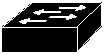
\includegraphics{switch.pdf}};
                            \node[onslide=<2->{white,opacity=0}] at (0,-0.6){B:1};
                            \node[onslide=<1>{white,opacity=0}] at (0,-0.6){B:3};
                        \end{tikzpicture}
                    }
                };

                \draw
                (A) -- (C)
                (C) -- (D)
                (B) -- (D)
                (D) -- (client);

                \draw [red, thick, dashed, onslide=<2->{white}]
                (A) -- (B);
            \end{tikzpicture}
        \end{figure}
    \end{minipage}%
    \begin{minipage}{.5\textwidth}
        \begin{enumerate}[<+(2)->]
            \item Vergleiche alle Bridges mit allen anderen
            \item Entferne Duplikate mit höherer Message Age
        \end{enumerate}
        \pause
        Dadurch bleiben alle korrekten Pfade erhalten
    \end{minipage}
\end{frame}

\begin{frame}{Visualisierung}
    \centering
    \begin{tikzpicture}[]
        \node[white,onslide=<2->{black}] (0) at (7.000000,20) {Root};
        \node[white,onslide=<3->{black}] (1) at (2.333333,18) {A, 1};
        \node[white,onslide=<4->{black}] (3) at (7.000000,18) {B, 1};
        \node[white] (4) at (11.666667,18) {};
        \node[white,onslide=<5->{black}] (2) at (11.666667,16) {C, 2};

        \draw[white,onslide=<7->{black}] (0) -- (1);
        \draw[white,onslide=<7->{black}] (0) -- (3);
        \draw[white,onslide=<7->{black}] (0) -- (4);
        \draw[white,onslide=<6->{black}] (4) -- (2);
    \end{tikzpicture}
\end{frame}

\begin{frame}{}
    \centering
    \huge \alert{Testen?}
\end{frame}

\begin{frame}{Überblick}
    \begin{itemize}
        \item \textbf{Einleitung \& Motivation}
        \item \textbf{Spanning Tree Protocol (STP)}
        \item \textbf{STPViz}
        \item \alert{\textbf{Software-Switch}}
        \item \textbf{Tests}
        \item \textbf{Zusammenfassung \& Ausblick}
    \end{itemize}
\end{frame}

\begin{frame}{Software-Switch}
    \begin{itemize}[<+->]
        \item STP Implementation in OpenWrt und dd-wrt fehlerhaft
        \item Emuliert STP fähige Bridge
        \item Multithreaded (POSIX Threads)
        \item \alert<7>{Probleme mit NetworkManager}
        \item Nicht sehr ausgiebig getestet
    \end{itemize}
\end{frame}

\begin{frame}{Überblick}
    \begin{itemize}
        \item \textbf{Einleitung \& Motivation}
        \item \textbf{Spanning Tree Protocol (STP)}
        \item \textbf{STPViz}
        \item \textbf{Software-Switch}
        \item \alert{\textbf{Tests}}
        \item \textbf{Zusammenfassung \& Ausblick}
    \end{itemize}
\end{frame}

\begin{frame}{Setup}
    \begin{figure}[h]
        \begin{center}
            \begin{tikzpicture}[scale=0.8]
                \node (root) at (2, 4) {\switch{0.6}{Root}};
                \node (a) at (0, 2) {\switch{0.6}{Bridge A}};
                \node (na) at (-1, 0.5) {Node A};
                \node (b) at (4, 2) {\switch{0.6}{Bridge B}};
                \node (nb) at (5, 0.5) {Node B};
                \node (c) at (2, 0) {\switch{0.6}{Bridge C}};
                \node (nc) at (2, -1.5) {Node C};
                \draw 
                (root) -- (a)
                (root) -- (b)
                (a) -- (c)
                (a) -- (na)
                (b) -- (nb)
                (c) -- (nc);

                \draw[onslide=<2>{white}]
                (b) -- (c);
            \end{tikzpicture}
        \end{center}
    \end{figure}
\end{frame}

\begin{frame}{Physisches Setup}
    \begin{figure}
        \centering
        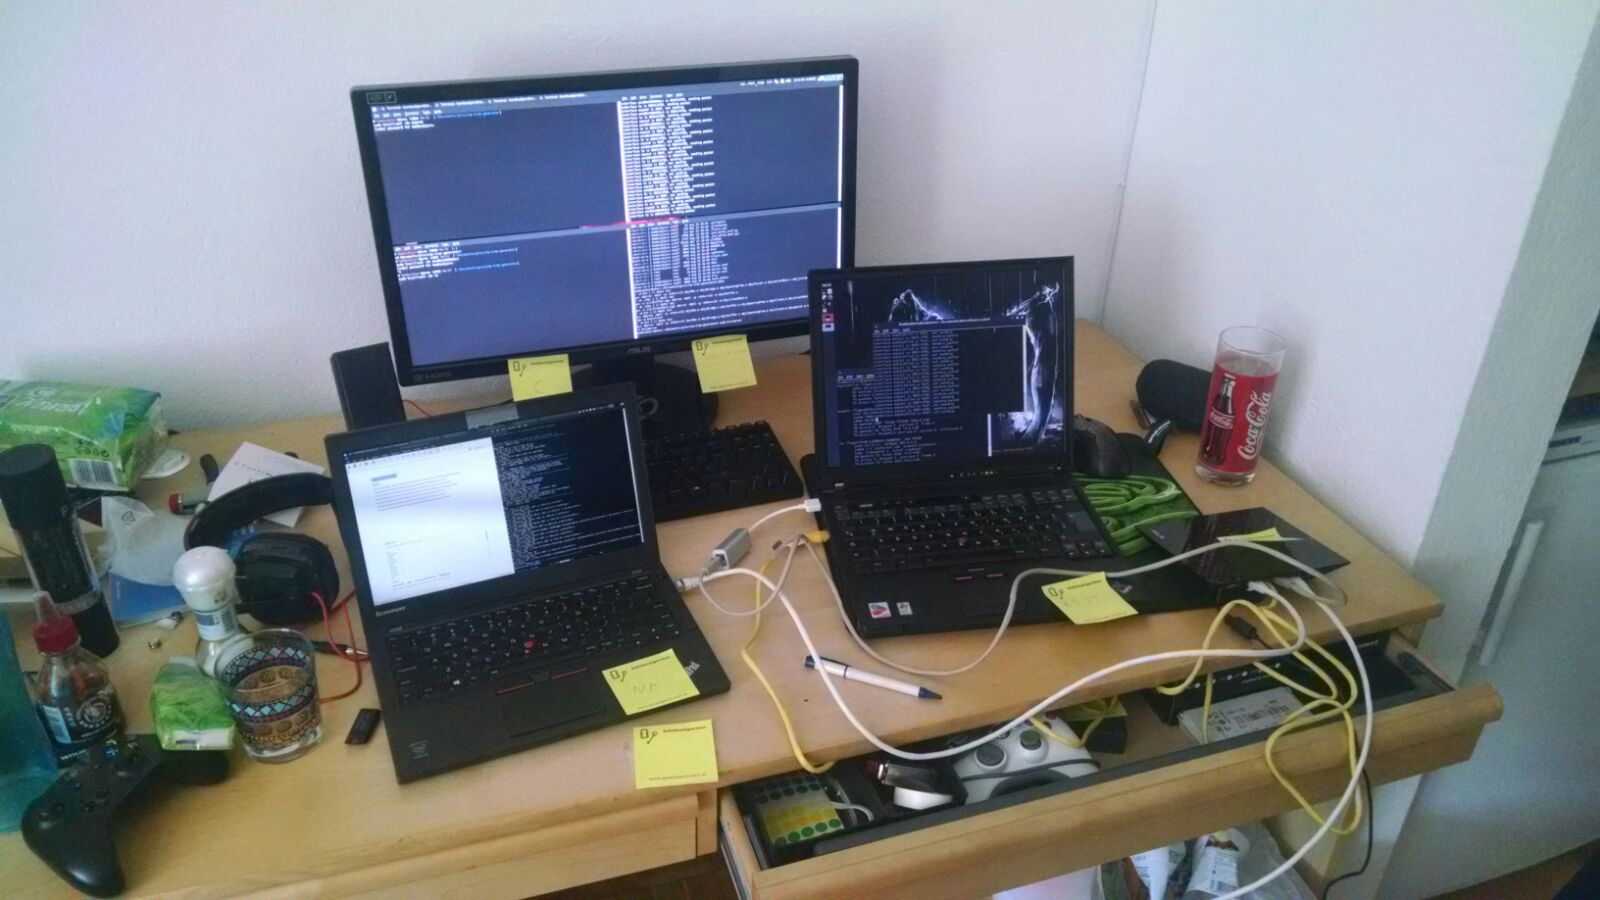
\includegraphics[width=\textwidth]{physicalSetup}
    \end{figure}
\end{frame}

\begin{frame}{Plug and Play Test}
    Verbindung wird hergestellt, bevor STPViz gestartet wird\\
    \pause
    \vspace{0.3cm}
    \centering
    \scalebox{0.8}{
        \begin{tikzpicture}[]
\node (0) at (7.000000,20) {32768:0 - BC:AE:C5:EB:7D:B6, 0};
\node (1) at (2.333333,18) {32768:1 - 00:E1:00:00:0D:C4, 1};
\node (2) at (7.000000,18) {};
\node (3) at (7.000000,16) {32768:0 - F4:F2:6D:7D:BF:BD, 2};
\draw (2) -- (3);
\node (4) at (11.666667,18) {32768:1 - 00:E0:7C:C8:57:E7, 1};
\draw 
(0) -- (1)
(0) -- (2)
(0) -- (4);
\end{tikzpicture}

    }
\end{frame}

\begin{frame}{Tree Establishment Test}
    STPViz wird gestartet, bevor Verbindung hergestellt wird\\
    \pause
    \vspace{0.3cm}
    \centering
    \scalebox{0.8}{
        \begin{tikzpicture}[]
\node (0) at (7.000000,20) {32768:0 - BC:AE:C5:EB:7D:B6, 0};
\node (1) at (3.500000,18) {32768:1 - 00:E0:7C:C8:57:E7, 1};
\node (2) at (3.500000,16) {61440:0 - F4:F2:6D:7D:BF:BD, 2};
\draw 
(1) -- (2);
\node (3) at (10.500000,18) {32768:1 - 00:E1:00:00:0D:C4, 1};
\draw 
(0) -- (1)
(0) -- (3);
\end{tikzpicture}

    }
\end{frame}

\begin{frame}{Dynamische Tests}
    (Physische) Topologie wird nach der Erkennung verändert\\
    \vspace{0.3cm}
    \centering
    \only<1-2>{
        \begin{tikzpicture}
            \node (root) at (2, 4) {\switch{0.8}{Root}};
            \node (a) at (0, 2) {\switch{0.8}{A}};
            \node (b) at (4, 2) {\switch{0.8}{B}};
            \node (c) at (2, 0) {\switch{0.8}{C}};

            \draw
            (root) -- (b)
            (a) -- (c);

            \draw[onslide=<2>{white}]
            (b) -- (c)
            (root) -- (a);

            \draw[white, onslide=<2>{black}]
            (a) -- (b);
        \end{tikzpicture}
    }
    \only<3>{
        \scalebox{0.8}{
            \begin{tikzpicture}[]
\node (0) at (7.000000,20) {32768:0 - BC:AE:C5:EB:7D:B6, 0};
\node (1) at (7.000000,18) {};
\node (2) at (7.000000,16) {32768:1 - 00:E0:7C:C8:57:E7, 2};
\node (3) at (7.000000,14) {61440:0 - F4:F2:6D:7D:BF:BD, 3};
\draw 
(2) -- (3);
\draw (1) -- (2);
\draw 
(0) -- (1);
\end{tikzpicture}

        }
    }
\end{frame}

\begin{frame}{Überblick}
    \begin{itemize}
        \item \textbf{Einleitung \& Motivation}
        \item \textbf{Spanning Tree Protocol (STP)}
        \item \textbf{STPViz}
        \item \textbf{Software-Switch}
        \item \textbf{Tests}
        \item \alert{\textbf{Zusammenfassung \& Ausblick}}
    \end{itemize}
\end{frame}

\begin{frame}{Ergebnisse}
    STPViz kann:
    \begin{enumerate}[<+(1)->]
        \item Bridges mit ihrer Entfernung zur Root erkennen
        \item Lokale Information zu globaler zusammenbauen
        \item Fehler korrigieren
        \item Diese Information sinnvoll visualisieren
    \end{enumerate}
    \pause
    STPViz kann nicht:
    \begin{enumerate}[<+(1)->]
        \item Features von STP Erweiterungen nutzen
        \item Kabeltypen bestimmen
        \item Nur notwendige Informationen verwerfen
        \item Topologien direkt aus \textit{.pcapng} Dateien erstellen
    \end{enumerate}
    \pause
    \alert{Kann nicht mit kommerziellen Tools mithalten, ist aber auch nicht nutzlos.}
\end{frame}

\begin{frame}{Zeitplanung}
    \centering
    \begin{figure}
        \begin{tikzpicture}[month]
            \draw (0,0) -- (0.4,0);
            \draw[->] (0.6,0) -- (10,0);
            %cut marker
            \draw[decorate, decoration={snake,amplitude=1pt,segment length=5pt}] (0.41, 0.3) -- (0.41, -0.3);
            \draw[decorate, decoration={snake,amplitude=1pt,segment length=5pt}] (0.62, 0.3) -- (0.62, -0.3);
            \foreach \x in {0,...,9}
                \draw (\x,0.1) -- (\x,-0.1);

            \node at (0,-0.5) {\tiny Oktober};
            \node at (1,-0.5) {\tiny Februar};
            \node at (2,-0.5) {\tiny März};
            \node at (3,-0.5) {\tiny April};
            \node at (4,-0.5) {\tiny Mai};
            \node at (5,-0.5) {\tiny Juni};
            \node at (6,-0.5) {\tiny Juli};
            \node at (7,-0.5) {\tiny August};
            \node at (8,-0.5) {\tiny September};
            \node at (9,-0.5) {\tiny Oktober};

            \draw (0,0.7) rectangle (1,0.5);\node () at (0.5,1) {\tiny Vorarbeit}; 
            \draw (1,0.7) rectangle (3,0.5);\node () at (2,1) {\tiny Implementation}; 
            \draw (3,0.7) rectangle (3.5,0.5);\node () at (3.25,1) {\tiny Tests};
            \draw (3.5,0.7) rectangle (4.5,0.5);\node () at (4,1) {\tiny Zus. Feat.}; 
            \draw (4.5,0.7) rectangle (5,0.5);\node () at (4.75,1) {\tiny Tests};
            \draw (5,0.7) rectangle (6,0.5);\node () at (5.5,1) {\tiny Arbeit}; 
            \draw[->] (6,1.5) -- (6,0);\node () at (6,1.7) {\tiny Präsentation};
        \end{tikzpicture}
    \end{figure}
    \vspace{0.3cm}
    \pause
    \begin{figure}
        \begin{tikzpicture}[month]
            \draw (0,0) -- (0.4,0);
            \draw[->] (0.6,0) -- (10,0);
            %cut marker
            \draw[decorate, decoration={snake,amplitude=1pt,segment length=5pt}] (0.41, 0.3) -- (0.41, -0.3);
            \draw[decorate, decoration={snake,amplitude=1pt,segment length=5pt}] (0.62, 0.3) -- (0.62, -0.3);
            \foreach \x in {0,...,9}
                \draw (\x,0.1) -- (\x,-0.1);

            \node at (0,-0.5) {\tiny Oktober};
            \node at (1,-0.5) {\tiny Februar};
            \node at (2,-0.5) {\tiny März};
            \node at (3,-0.5) {\tiny April};
            \node at (4,-0.5) {\tiny Mai};
            \node at (5,-0.5) {\tiny Juni};
            \node at (6,-0.5) {\tiny Juli};
            \node at (7,-0.5) {\tiny August};
            \node at (8,-0.5) {\tiny September};
            \node at (9,-0.5) {\tiny Oktober};

            \draw (0,0.7) rectangle (1,0.5);\node () at (0.5,1) {\tiny Vorarbeit}; 
            \draw (1,0.7) rectangle (6,0.5);\node () at (3.5,1) {\tiny STPViz}; 
            \draw (6,0.7) rectangle (7,0.5);\node () at (6.5,1) {\tiny Soft-Switch};
            \draw (7,0.7) rectangle (8,0.5);\node () at (7.5,1) {\tiny Testen}; 
            \draw (8,0.7) rectangle (9.1,0.5);\node () at (8.5,1) {\tiny Arbeit};
            \draw[->] (9.5,1.5) -- (9.5,0);\node () at (9.5,1.7) {\tiny Präsentation};
        \end{tikzpicture}
    \end{figure}

\end{frame}

\begin{frame}{Ausblick}
    Sinnvolle nächste Schritte:
    \begin{enumerate}[<+(1)->]
        \item Features von STP Erweiterungen nutzen
        \item Kabeltypen bestimmen
        \item Nur notwendige Informationen verwerfen
        \item Topologien direkt aus \textit{.pcapng} Dateien erstellen
        \item STP Implementation in OpenWrt und dd-wrt verbessern
        \item Software-Switch voll funktionstüchtig machen
    \end{enumerate}
\end{frame}

\begin{frame}{Code}
    Code und Arbeit sind verfügbar unter:\\
    \vspace{0.5cm}
    https://github.com/alxshine/stp-tree-generator\\
    https://github.com/alxshine/software-switch
\end{frame}

\end{document}
